\chapter{Functional programming} 
\vspace{-1cm}
Functional programming is a programming paradigm 
to mimic mathematical functions. 
It can be considered a declarative programming language 
that builds complex functions by functional composition. 
Functional Programming is based on Lambda Calculus developed 
by Alonzo Church (1903-1995). 
Alan Turing (1912-1954), who was a student of Alonzo Church, created the 
universal Turing machine which laid the foundation of imperative 
programming style.
Python and Fortran both support functional programming in some degree.  
In this chapter, the following concepts, associated to functional 
programming, will be discussed through  different examples 
for Python and Fortran:  
\begin{enumerate} 
 \setlength\itemsep{0cm}
\item First-Class functions.
\item Pure functions and side effects.
\item Recursion. 
\item Map, filter and reduce elemental functions.  
\item Modularity. 
\item Closure.
\item Referential transparency. 
\end{enumerate} 
Main advantages of functional programming are: its closeness 
to mathematical formulation, its ability to avoid side effects and 
its modularity to partition complex problems into easier ones.
One of main disadvantages is a lower  computational performance 
than imperative paradigm associated to recursion and functional composition
techniques.  Functional programming is usually used in mathematical 
computations and when parallelism or concurrency is required.


 
\newpage
 \section{First-class functions} 
A programming language has first-class functions 
when functions can be treated like any other variable. 
Namely, functions can be used in the following situations:  
\begin{enumerate} 
\item Function with arguments that are also functions.
\item Functions returning functions. 
\item Functions being assigned to other functions.
\end{enumerate} 

\subsection{Functions as arguments} 
Many mathematical concepts or functions are defined for a 
specific set of functions.
For example, the integral of some function is defined by: 
\begin{equation}
 I = \int _a ^b f(x)  \ dx, \qquad f: \mathbb{R} \rightarrow \mathbb{R}
\end{equation} 
It is desirable to implement a function to determine the definite integral
in the compact segment $ [a, b ]$ for any  
$  f: \mathbb{R} \rightarrow \mathbb{R} $. 
In order to have a complete example, an approximate method is needed to 
define the integral. Let's consider the right Riemann sum 
as an approximation by a finite sum: 
\begin{equation}
 I \approx \sum _{i=1} ^N f(x_i)  \ ( x_i - x_{i-1} ),
\end{equation}
where $ x_i $ is a partition of $ [a, b]$ 
\begin{equation}
 a = x_0 < x_1  < \cdots < x_N = b.
\end{equation}
In the following scheme, the interface of function integral is defined:  

\begin{center} 
 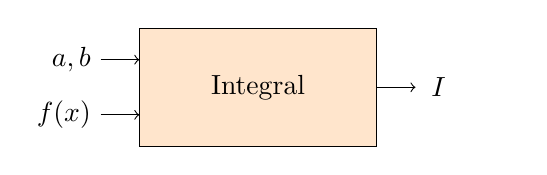
\begin{tikzpicture}
 \node[draw, fill=orange!20, minimum height=1.5cm, minimum width=3cm] (node) at (0,0) {Integral};
 \draw[->] (-2,0.35)node[anchor=east] {$a,b$} to (\tikztostart -| node.west);
 \draw[->, black] (-2,-0.35) node[anchor=east] {$f(x)$} to (\tikztostart -| node.west);
 \draw[->]  (1.5,0) node  {} to (2,0);
 \node[text width=1cm] at (2.7,0) {$I$};
 \end{tikzpicture}
\end{center} 



  
 \newpage 
  \subsubsection*{Fortran} 
The main purpose is to write a function with three arguments. The two first
are real numbers: $ a $ and $ b$. 
The interface definition of third argument  
$( f: \mathbb{R} \rightarrow \mathbb{R} ) $
is expressed with the following code:  
\vspace{0.5cm} 
   \renewcommand{\home}{./Fortran/sources/Advanced_programming/functional programming} 
   \lstfor
  \listings{\home/First_class_functions.f90}{abstract interface}
  {end interface}{First_class_functions.f90}
Once every argument is defined, the function integral is implemented: 
%  \listings{\home/First_class_functions.f90}{subroutine Function_examples}
%  {end subroutine}{First_class_functions.f90}
 \vspace{0.3cm}  
 % \newpage 
  \listings{\home/First_class_functions.f90}{real function Integral}
  {end function}{First_class_functions.f90}
Note that the third argument is a procedure function defined above. 
The following example creates a function $ h(x) $ to be integrated 
using the new function \verb|Integral|. 
 \vspace{0.3cm}  
  \listings{\home/First_class_functions.f90}{real function h}
   {end function}{First_class_functions.f90}
 
\newpage
\subsubsection*{Python}
Since Python is untyped language, 
\verb|Integral| function is implemented without specifying the type of its
arguments with the following code: 
\renewcommand{\home}{./Python/sources/Advanced_programming/functional programming}
\lstpython 
\vspace{0.5cm}
\listingsp{\home/First_class_functions.py}{def Integral}
  {return}{First_class_functions.py}
Note that the extension of the \verb|Integral| function has been reduced 
drastically by sacrificing 
the specifications or variables and arguments. 
Once someone makes use of this function, the Python interpreter will 
check dynamically that the operations involved in the above code 
are defined.
If the function $ h(x) $ is defined by: 
\vspace{0.5cm}
\listingsp{\home/First_class_functions.py}{def h}
  {return}{First_class_functions.py}
by invoking 
\vspace{0.5cm}
\listingsp{\home/First_class_functions.py}{R = Integral}
  {print}{First_class_functions.py}
will work without any problem.    

\newpage 
\subsection{Functions returning functions} 
In mathematics, 
function composition is an operation 
that takes two functions $f$ and $g$, and yields a function $ h = g  \circ  f  $ 
such that $ h(x) = g(f(x))$. 
Once the image of $ x $ is obtained by applying the function $ f $, 
a new image  $g(f(x))$ is yielded by applying $ g $. 

In Fortran language, functions can not return functions. 
The only possibility is to create derived types comprising 
functions or procedure pointers. This strategy is closer to the
Object Oriented Programming and it will treated in next chapters. 
However, Python allows very intuitively to build functions returning functions. 

\subsubsection*{Python}
The following example shows the definition of a function which returns 
the function composition of $ f $ and $ g $
\lstpython 
\vspace{0.5cm}
\listingsp{\home/First_class_functions.py}{def compose}
  {return h}{First_class_functions.py}
  
\subsection{Functions being assigned to other functions} 
Following with the same mathematical example, 
the creation of a new composition function is written in mathematical 
language as:
\begin{equation}
     h = f \circ g  
\end{equation} 
Fortran does not allow to assign functions to each other. 
The same strategy described above based on function or procedure pointer can be used to 
overcome this deficiency. However, Python allows to assign function
 as if they were variables as it is shown in the following code snippet: 
\lstpython 
\vspace{0.4cm}
\listingsp{\home/First_class_functions.py}{sqrt}
  {sqrt}{First_class_functions.py}




\newpage   
\section{Pure functions} 
In computer programming, a pure function is a function 
that returns values identical for identical arguments
and has no side effects. 
Hence, a pure function is a computational analogue of a mathematical function. 
Pure functions can be explicitly declared in Fortran with the \verb|pure| attribute.
However, in Python there is no way to force a function to be pure.  
The following list constitutes the requirements for a function to be pure.    
 \begin{enumerate}
  \setlength\itemsep{0.1cm}
 \item The function must not alter any dummy argument. 
 To accomplish that in Fortran,  arguments must have \verb|intent(in)| attribute 
 unless they are procedures or pointers.   
 \item The function must  not alter any part of a variable accessed by host or 
 use association. 
 \item Local variables can not have the \verb|SAVE| attribute(Fortran) or be saved. 
 \item Functions as arguments must be pure. 
 \item No external input/outputs operations are allowed. 
 \item STOP is not allowed. 
 \end{enumerate}   
If the Fortran function is declared with the \verb|pure| attribute and any of those 
requirements are not fulfilled, the compilation process of the source code will prompt an error.
In Python if pure functions are required, special care should be taken into account with these 
requirements. 
Those requirements are needed to assure that pure functions returns 
the same values for identical input arguments. 
One of main characteristics of any software development strategy is data hiding. It means that
non necessary data should be hidden to avoid bugs or improper behavior. 
However, when external data or global variables are needed, 
pure functions must not modify those variables. 

It seems that writing the entire code with pure functions would be our goal to improve 
efficiency in developing software. However, sometimes because a database should be modified 
or a random number generator is used, the same output is not obtained. 
The goal is to use pure functions when practical. Total purity 
is not practical but what about  80\% purity.


For sake of clarity, requirements to implement pure functions are  discussed in the following example: 
\newpage  
    \renewcommand{\home}{./Fortran/sources/Advanced_programming/functional programming} 
    \lstfor
   \listings{\home/First_class_functions.f90}{pure_functions}
   {end subroutine}{First_class_functions.f90}
The function \verb|f(x)| is declared to be pure. It has only one argument a real value \verb|x|.
As it was mentioned, \verb|x| must be specified with the \verb|intent(in)| attribute 
in order not to be modified accidentally.
A local variable \verb|b| is declared. This local variable can not have the \verb|SAVE| attribute
or can not be initialized to avoid undesirable historical effects. 
The function \verb|f_impure(x)| is impure because it has the initialization \verb|real::b=1|.
The first time this function is called with $ x=1$, it gives \verb|4,0| and the second time 
it yields \verb|5.0|. The reason is because the variable \verb|b| is only initialized at compilation 
time and saved for future calls. The first time \verb|f_impure(x)| is called, 
and after the sentence \verb|b=b+1|, variable \verb|b| holds \verb|2.0|. 
The second time \verb|f_impure(x)| is called, 
and after the sentence \verb|b=b+1|, variable \verb|b| holds \verb|3.0| and 
 \verb|f_impure(x)| gives a different value than the first call with identical input \verb|x|. 
Those are typical errors that can be avoided by writing  pure functions.

   


\newpage  
\section{Recursion}
\vspace{-0.5cm}  
In mathematics, a recursive definition or inductive definition, 
is used to define the elements in a set in terms of other elements in the set.
A recursive function is a function that its value at any point can be calculated 
from the values of the function at some previous points. 
For example,  the Fibonacci sequence 
\begin{equation} 
F(n) = F(n-1) + F(n-2)
\label{Fibonacci} 
\end{equation}
gives $ F(n) $ once $ F(n-1) $ and $F(n-2)$ are known. If the function values at  $n=0$  and 
$ n=1$ are known, the function value at $ n=2$ can be obtained from  the equation (\ref{Fibonacci}).
Recursive functions in programming languages allows to obtain the sequence 
from the declarative point of view. That is, it is not need to develop an iterative 
or imperative procedure as it is described above. 
As it was mentioned, recursive procedures are less efficient in terms of computational 
resources than iterative implementations. However, recursive implementations are easier to 
debug and to implement.  
 
\vspace{-0.5cm}
\subsection*{Fortran}
 \renewcommand{\home}{./Fortran/sources/Advanced_programming/functional programming} 
    \lstfor
   \listings{\home/First_class_functions.f90}{function Fibonacci}
   {end function}{First_class_functions.f90}
   \vspace{-0.8cm}
\subsection*{Python}
 \renewcommand{\home}{./Python/sources/Advanced_programming/functional programming} 
    \lstpython
   \listingsp{\home/First_class_functions.py}{def Fibonacci}
   {n-2}{First_class_functions.py}
   
   
 
  
\newpage  
\section{Map, filter and reduce}

In mathematics, mapping refers to the action of applying a function to the elements of its domain.
Mapping applies to any set: a collection of objects. 
\begin{equation} 
   f:A \rightarrow B 
\end{equation}    
is a map from $ A $ to $ B$; for every 
$ a $  in $ A$, there is a unique object $ f(a)$  in $ B$.
For example, rotating 
a body about a point is map that transform the body coordinates into new coordinates 
keeping the axes fixed. 


A filter on a set $ X $ is 
a special family of subsets. A filter on a set may be thought 
of as representing a "collection of large subsets".
Filters in topology can be used to study topological spaces 
and define all basic topological notions such a 
convergence, continuity, compactness, and more.
One of the first examples of a filter is the neighborhood filter 
$\mathcal{N}(x) $ at a point 
$ x$  in a topological space 
$(X,\tau )$ 
which is the family of sets consisting of all neighborhoods of $x$.  
By definition, a neighborhood of some given point $x$  
is any subset $  B \subseteq X $ 
whose topological interior contains this point; 
that is, such that $ x \in \operatorname {Int} _{X}B.$





\vspace{1cm} 
\begin{IN}
The mathematical concepts: map/filter/reduce allow a software design 
simplifying the implementation of functions that operate over sequences of elements
enabling an implementation with no explicit control flow, not a single loop or if statements.
\end{IN}
\vspace{0.5cm} 
These mathematical concepts are taken into account in a functional programming language 
such as Python and Fortran and they will be explained in the following sections through examples.







\newpage 
\subsection{Mapping} 
To explain the implementation of the map functionality, let's consider a rotation 
which is a map of a plane into itself. The rotated coordinates of the point $(x,y)$ with an angle 
$\theta$ are: 
\begin{equation}
\begin{pmatrix}
x_r \\
y_r
\end{pmatrix}
=
\begin{pmatrix}
cos \ \theta & -sin \ \theta\\
sin \ \theta &  cos \ \theta
\end{pmatrix}
\begin{pmatrix}
x \\
y
\end{pmatrix}
\label{rotation} 
\end{equation} 
In the following example a square is rotated $ \pi/4 $ radians.
\subsubsection*{Fortran}
\renewcommand{\home}{./Fortran/sources/Advanced_programming/functional programming} 
  \lstfor
 \listings{\home/map_filter_reduce.f90}{type :: point2D}
 {end type}{map_filter_reduce.f90}
 \listings{\home/map_filter_reduce.f90}{function Rotation}
  {end function}{map_filter_reduce.f90}
\listings{\home/map_filter_reduce.f90}{image =}
  {imageR =}{map_filter_reduce.f90}  
First, the new type \verb|point2D| is defined. It is determined by its $ (x,y)$ coordinates. 
Then, rotation equation (\ref{rotation}) is implemented in \verb|Rotation|.
Finally, a set of  \verb|point2D| points is mapped with the \verb|Rotation| function which is written 
for a generic \verb|point2D| point. Note that the attribute \verb|elemental| of this function allows
to apply this functions for isolated elements or for a whole set of points. 

\subsubsection*{Python}
\renewcommand{\home}{./Python/sources/Advanced_programming/functional programming}
 \lstpython
 \listingsp{\home/map_filter_reduce.py}{def Rotation}
  {return}{map_filter_reduce.py}
  \vspace{0.5cm} 
\listingsp{\home/map_filter_reduce.py}{image =}
  {imageR =}{map_filter_reduce.py}  
Since Python is an untyped langauage, there is no need to define the plane point \verb|P|.
Hence,  \verb|Rotation| function is implemented assuming that \verb|P| is an numpy array with 
two components. This is assumed from expression \verb|matmul(A, P)|. 
Since \verb|A| is a square matrix of dimension 2, \verb|P| should be a vector of dimension 2 
 to have a conformal operation. 
 
Finally, a set of points is mapped with the \verb|Rotation| function which is written 
for a generic point. Note that the keyword \verb|map| allows this mapping. 
The first argument of \verb|map| is the scalar function to be applied to each element 
of the set and the second argument is the set. Since \verb|Rotation| has two arguments: 
point and angle to be rotated, a \verb|lambda| function is used to define a 
new function with of only one argument.  



  
  
 \newpage 
\subsection{Filter}   
  
 \newpage 
 \subsection*{Fortran} 
 \renewcommand{\home}{./Fortran/sources/Advanced_programming/functional programming} 
  \lstfor
 \listings{\home/map_filter_reduce.f90}{subroutine test_map_filter_reduce}
 {end subroutine}{map_filter_reduce.f90}
  
 \listings{\home/map_filter_reduce.f90}{elemental integer function str_to_number}
 {end function}{map_filter_reduce.f90}
 
 
 \newpage 
 \subsection*{Python}
 \renewcommand{\home}{./Python/sources/Advanced_programming/functional programming}
 \lstpython
 \listingsp{\home/map_filter_reduce.py}{def test_map_filter_reduce}
 {max value}{map_filter_reduce.py}
 \listingsp{\home/map_filter_reduce.py}{def str_to_number}
 {return}{map_filter_reduce.py}
 
 


Named parameters and default parameters  

\newpage   
\section{Modularity} 


 
  The only input to a pure function is its argument list and the only output is its return value. 
  If you haven’t seen this before, you might 
  think all functions are pure. After all, any function takes in values and returns a value.
   But in conventional programming there are 
  typically out-of-band ways for information to flow in or out of a function. 
  For example, an impure function may depend on a global variable 
  or class member data. 
  In that case, it’s behavior is not entirely determined by its arguments. Similarly, an impure function might set a 
  global variable or write to a database. 
  In that case the function has a side effect in addition to its return value.
  
  You can write pure functions in any language, 
  though it’s easier in some languages than others. 
  For example, no one would call Fortran a 
  functional language, but there are people (M. J. D. Powell comes to mind)
   who discipline themselves to write pure functions in Fortran.
  
  
  
  
  So why don’t programmers use pure functions more often? 
  One reason is that pure functions require longer argument lists. 
  In an object 
  oriented language, object methods can have shorter argument lists 
  by implicitly depending on object state. 
  The price to pay for shorter 
  method signatures is that you can’t understand a method by itself. 
  You have to know the state of the object when the method is called. 
  Is 
  it worthwhile to give up referential transparency in order to have shorter method signatures? 
  It depends on your context and your taste, 
  though in my opinion its often worthwhile to use longer function 
  signatures in exchange for more pure functions.
  
  Another reason people give for not writing pure functions 
  is that its too expensive to copy large data structures to pass them into a 
  function. But that’s what pointers are for. You can conceptually 
  pass an object into a function without having to actually make a copy of 
  the object’s bits.
  
  You can also fake purity for the sake of efficiency. 
  For example, Mike Swaim left a comment recently giving an example of how memoization 
  sped up a program by several orders of magnitude. 
  (Memoization is a technique of caching computations. When a function is asked to compute 
  something, it first looks to see whether it has already done the calculation. If so, it returns the cached value. If not, it does the 
  calculation and adds its output to the cache.) 
  
  A function that uses memoization is not strictly pure — 
  its calculations have a persistent 
  impact on the state of its cache —
   but such a function can still have referential transparency, always returning the same output given the 
  same input. 
  You could say it’s cheating to call such functions pure, 
  and it is, but if you’re really a stickler about it, all pure 
  functions have side effects.
  
  

 
 
 









 In particular, in computer science, modular structure is typically held to
 support understandability, reliability, the possibility of independent development, flexibility, and reuse. Transferring notions of 
 modularity to mathematics
 provides insight as to how these benefits are achieved in that setting as well.
 This perspective is largely orthogonal to traditional approaches to addressing ontological and epistemological questions. In particular, it 
 seems equally
 compatible with realist and antirealist views of mathematics. But in addition
 to being independently valuable, a better understanding of what we value in
 mathematics, and why, can inform traditional lines of inquiry as well. For example, it can provide a more robust picture of how our 
 mathematical language
 deals with mathematical objects, and what it is about such objects that gives
 them the air of reality
 
 
 
 Modular programming (also referred to as modular architecture) is a general programming concept. It involves separating a program's 
 functions into independent pieces or building blocks, each containing all the parts needed to execute a single aspect of the functionality
 
 Modular programming is a software design technique that emphasizes separating the functionality of a program into independent, 
 interchangeable modules, such that each contains everything necessary to execute only one aspect of the desired functionality.
 
 A module interface expresses the elements that are provided and required by the module. The elements defined in the interface are detectable 
 by other modules. The implementation contains the working code that corresponds to the elements declared in the interface. Modular 
 programming is closely related to structured programming and object-oriented programming, all having the same goal of facilitating 
 construction of large software programs and systems by decomposition into smaller pieces, and all originating around the 1960s. While the 
 historical usage of these terms has been inconsistent, "modular programming" now refers to the high-level decomposition of the code of an 
 entire program into pieces: structured programming to the low-level code use of structured control flow, and object-oriented programming to 
 the data use of objects, a kind of data structure.
 
 In object-oriented programming, the use of interfaces as an architectural pattern to construct modules is known as interface-based 
 programming.[c
 
 
 CODING FORTRAN: INTERFACE BLOCKS (MODULARITY)
 03/02/2021
 Interface blocks provide a means of doing type checking between the calling subprogram, and the called subprogram. Incorrect types between 
 the calling arguments, and the subprogram parameters is a common source of problems. This doesn’t happen as much in languages such as C, 
 because if a real parameter is given as an argument to a subprogram which expects an integer it is merely truncated. Why use an interface 
 block? Largely because it is good programming practice to include explicit interfaces, even if they are not required.
 
 
 
 
  
\newpage  
\section{Closure} 

 
 \newpage 
  \renewcommand{\home}{./Fortran/sources/Advanced_programming/functional programming} 
  \listings{\home/First_class_functions.f90}{real function Moment}
  {end function}{First_class_functions.f90}
  

 and lexical scoping


Lexical scoping defines how variables are seen in nested functions.
When functions are defined inside other functions, the scope of this inner 
function comprises local variables of the actual function and 
local variables of those outer or parent functions.


 
inner functions contain the scope 
of parent functions even if the parent function has returned.
 


\newpage  
\section{Referential transparency}  


  Why write pure functions? A pure function has referential transparency, meaning it will always return the same value when given the same 
  inputs. The output does not depend on the system time, the state of a database, which functions were called previously, or anything else 
  that is not explicitly passed as an argument to the function. This means pure functions are easier to understand (and hence easier to debug 
  and test).



Pure functions are easier to understand because 
they don’t change any states and depend only on the input given to them. 
Whatever output they 
produce is the return value they give. 
Their function signature gives all the information 
about them i.e. their return type and their 
arguments.
The ability of functional programming languages to treat functions as values and pass them to functions as parameters make the code more 
readable and easily understandable.

Testing and debugging is easier. 
Since pure functions take only arguments and produce output, they don’t produce any changes don’t take input 
or produce some hidden output. 

They use immutable values, 
so it becomes easier to check some problems in programs 
written uses pure functions.

It is used to implement concurrency/parallelism because pure functions 
don’t change variables or any other data outside of it.
It adopts lazy evaluation which avoids repeated evaluation
because the value is evaluated and stored only when it is needed.



  
  
  